\documentclass[tikz,border=8pt]{standalone}
\usepackage{amsmath}
\usetikzlibrary{arrows.meta,calc,decorations.pathreplacing}
\definecolor{ink}{HTML}{21352F}
\definecolor{teal}{HTML}{087F7B}
\definecolor{blue}{HTML}{4B77A8}
\definecolor{gold}{HTML}{C58B2A}
\definecolor{rose}{HTML}{B65A62}
\begin{document}
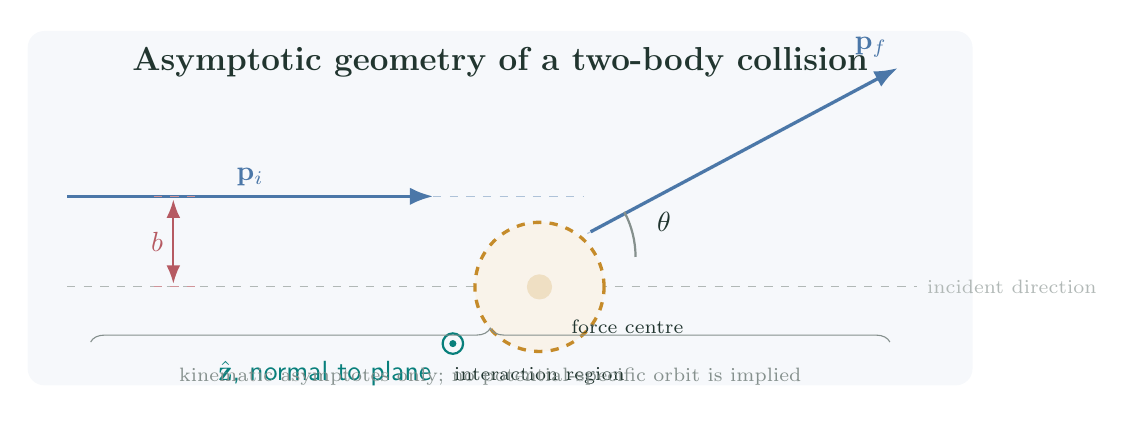
\begin{tikzpicture}[font=\sffamily,text=ink,>=Latex]
  \fill[blue!5,rounded corners=6pt]
    (-6.5,-1.25) rectangle (5.5,3.25);
  \node[font=\bfseries\large] at (-.5,2.85)
    {Asymptotic geometry of a two-body collision};

  \coordinate (O) at (0,0);
  \draw[ink!35,dashed] (-6,0)--(4.8,0)
    node[right,font=\scriptsize] {incident direction};
  \draw[blue,very thick,->] (-6,1.15)--(-1.35,1.15)
    node[midway,above] {$\mathbf p_i$};
  \draw[blue!45,dashed] (-1.35,1.15)--(.55,1.15);
  \draw[blue!45,dashed] (.05,.38)--(1.1,.94);
  \draw[blue,very thick,->] (.65,.7)--(4.55,2.78)
    node[above left] {$\mathbf p_f$};

  \fill[gold!10] (O) circle (.82);
  \draw[gold,very thick,dashed] (O) circle (.82);
  \fill[gold!28] (O) circle (.16);
  \node[font=\scriptsize,anchor=north west] at (.28,-.3)
    {force centre};
  \node[font=\scriptsize,anchor=north] at (0,-.9)
    {interaction region};

  \draw[<->,rose,thick] (-4.65,.04)--(-4.65,1.11)
    node[midway,left] {$b$};
  \draw[rose!65,dashed] (-4.9,1.15)--(-4.35,1.15);
  \draw[rose!65,dashed] (-4.9,0)--(-4.35,0);

  \draw[teal,thick] (-1.1,-.72) circle (.13);
  \fill[teal] (-1.1,-.72) circle (.045);
  \node[teal,anchor=north east] at (-1.25,-.82)
    {$\hat{\mathbf z}$, normal to plane};

  \draw[ink!55,thick] (1.22,.38)
    arc[start angle=0,end angle=28,radius=1.22];
  \node at (1.58,.83) {$\theta$};

  \draw[decorate,decoration={brace,amplitude=5pt},ink!55]
    (-5.7,-.7)--(4.45,-.7)
    node[midway,below=6pt,font=\scriptsize]
    {kinematic asymptotes only; no potential-specific orbit is implied};
\end{tikzpicture}
\end{document}
